% arara: pdflatex
% arara: biber
% arara: pdflatex
% arara: pdflatex
% arara: clean: { files: [radioemission.log,radioemission.aux,radioemis1sion.blg,radioemission.bbl,radioemission.bcf,radioemission.toc,radioemission.run.xml,radioemission.out ] }
% zsh> setopt no_nomatch

% Chandra Images by Category: Supernovas & Supernova Remnants
% https://chandra.harvard.edu/photo/category/snr.html

\documentclass[a4paper,12pt]{extarticle}

\RequirePackage[l2tabu,orthodox]{nag} % Раскомментировав, можно в логе получать рекомендации относительно правильного использования пакетов и предупреждения об устаревших и нерекомендуемых пакетах
% \documentclass[a4paper,14pt]{extarticle}
\usepackage[left=1.5 cm,right=1.6cm,top=1.5cm,bottom=2.5cm]{geometry}

%%% Mathematical packages %%%
\usepackage{amsthm,amsmath,amscd} % Математические дополнения от AMS
\usepackage{amsfonts,amssymb}     % Математические дополнения от AMS
\usepackage{mathtools}            % Добавляет окружение multlined
\usepackage{mathtext}
\usepackage{cancel}

\usepackage{textcomp}

\RequirePackage{ifxetex, ifluatex}
\ifxetex
  % https://tex.stackexchange.com/a/38631
  \renewcommand{\mathbf}{\ensuremath{\symbf}}
  \usepackage{unicode-math}
  \usepackage{polyglossia}                        % Поддержка многоязычности (fontspec подгружается автоматически)
 % \setmainlanguage[babelshorthands=true]{russian} % Язык по-умолчанию русский с поддержкой приятных команд пакета babel
  \setotherlanguage{english}                      % Дополнительный язык = английский (в американской вариации по-умолчанию)
  % Семейство шрифтов Liberation (https://pagure.io/liberation-fonts)
  \setmonofont{LiberationMono}[Scale=0.87]        % моноширинный шрифт
  \newfontfamily\cyrillicfonttt{LiberationMono}[  % моноширинный шрифт для кириллицы
    Scale=0.87]
  \defaultfontfeatures{Ligatures=TeX}             % стандартные лигатуры TeX, замены нескольких дефисов на тире и т. п. Настройки моноширинного шрифта должны идти до этой строки, чтобы при врезках кода программ в коде не применялись лигатуры и замены дефисов
  \setmainfont{LiberationSerif}                   % Шрифт с засечками
  \newfontfamily\cyrillicfont{LiberationSerif}    % Шрифт с засечками для кириллицы
  \setsansfont{LiberationSans}                    % Шрифт без засечек
  \newfontfamily\cyrillicfontsf{LiberationSans}   % Шрифт без засечек для кириллицы

  % fake small capitals
  % https://tex.stackexchange.com/questions/55664/fake-small-caps-with-xetex-fontspec
  \makeatletter
  \newlength\fake@f
  \newlength\fake@c
  \def\textsc#1{%
    \begingroup%
    \xdef\fake@name{\csname\curr@fontshape/\f@size\endcsname}%
    \fontsize{\fontdimen8\fake@name}{\baselineskip}\selectfont%
    \MakeUppercase{#1}%
    \endgroup%
    }
  \makeatother
  % \renewcommand{\textsc}[1]{\fauxschelper#1 \relax\relax}
  % \def\fauxschelper#1 #2\relax{%
  %   \fauxschelphelp#1\relax\relax%
  %   \if\relax#2\relax\else\ \fauxschelper#2\relax\fi%
  %   }
  % \def\Hscale{.83}\def\Vscale{.72}\def\Cscale{1.00}
  % \def\fauxschelphelp#1#2\relax{%
  %   \ifnum`#1>``\ifnum`#1<`\{\scalebox{\Hscale}[\Vscale]{\uppercase{#1}}\else%
  %   \scalebox{\Cscale}[1]{#1}\fi\else\scalebox{\Cscale}[1]{#1}\fi%
  %   \ifx\relax#2\relax\else\fauxschelphelp#2\relax\fi}

\else
  \usepackage[T2A]{fontenc}           % кодировка
  \usepackage[utf8]{inputenc}         % Кодировка utf8
  \usepackage[english,russian]{babel} % Языки: русский, английский
\fi

\usepackage[colorlinks=true,unicode=true]{hyperref}

%%% Other packages %%%
\usepackage{xspace} % пробелы после предопределённых команд
\usepackage{color}
\usepackage{enumitem}
\usepackage{cmap}
\usepackage{array}
\usepackage{braket}
\usepackage{epsfig}
\usepackage{epstopdf}
\usepackage{graphicx}
\usepackage{float}
\usepackage{caption}
\captionsetup{compatibility=false}
\usepackage{subcaption}
\usepackage{indentfirst}
\usepackage{hyphenat}
\usepackage[normalem]{ulem}
\usepackage{wrapfig}
\usepackage{pdfpages}

\graphicspath{{img/}} % Пути к изображениям

%%% Toc %%%
% \setcounter{tocdepth}{4}
% \setcounter{secnumdepth}{4}

%%% Title %%%
% \usepackage{titlesec}
% \titleformat{\section}
% {\normalfont\large\bfseries}{\thesection}{1em}{}

%%% Setup bibliography %%%

\usepackage{csquotes} % biblatex рекомендует его подключать. Пакет для оформления сложных блоков цитирования.
%%% Загрузка пакета с основными настройками %%%
\makeatletter
\usepackage[%
backend=biber,% движок
bibencoding=utf8,% кодировка bib файла
sorting=none,% настройка сортировки списка литературы
style=gost-numeric,% стиль цитирования и библиографии (по ГОСТ)
language=autobib,% получение языка из babel/polyglossia, default: autobib % если ставить autocite или auto, то цитаты в тексте с указанием страницы, получат указание страницы на языке оригинала
autolang=other,% многоязычная библиография
clearlang=true,% внутренний сброс поля language, если он совпадает с языком из babel/polyglossia
defernumbers=true,% нумерация проставляется после двух компиляций, зато позволяет выцеплять библиографию по ключевым словам и нумеровать не из большего списка
sortcites=true,% сортировать номера затекстовых ссылок при цитировании (если в квадратных скобках несколько ссылок, то отображаться будут отсортированно, а не абы как)
movenames=false, % опция разрешает или запрещает перемещение имён в область сведений об ответственности, если количество имён больше трёх.
% не менять местами заголовок и список авторов, если авторов больше четырех
minnames=3, % сокращение списка имён
maxnames=4, % сокращение списка имён
doi=true,% Показывать или нет ссылки на DOI
isbn=false,% Показывать или нет ISBN, ISSN, ISRN
url=false,
eprint=true,
backref=true
]{biblatex}[2016/09/17]
%]{biblatex}
%\ltx@iffilelater{biblatex-gost.def}{2017/05/03}%
{\toggletrue{bbx:gostbibliography}%
\renewcommand*{\revsdnamepunct}{\addcomma}}{}
\makeatother

\DefineBibliographyStrings{english}{docthesis = {dissertation}}
\DefineBibliographyStrings{russian}{docthesis = {диссертация}}

% Custom backref Text
%https://tex.stackexchange.com/questions/196015/custom-backref-text
\DefineBibliographyStrings{english}{
  backrefpage  = {Цит. на с.\adddot},
  backrefpages = {Цит. на с.\adddot},
}
\DefineBibliographyStrings{russian}{
  backrefpage  = {Цит. на с.\adddot},
  backrefpages = {Цит. на с.\adddot},
}
\ifxetex
\else
% Исправление случая неподдержки знака номера в pdflatex
    \DefineBibliographyStrings{russian}{number={\textnumero}}
\fi

% разделитель ; для ссылок
\DeclareMultiCiteCommand{\multicites}[\mkbibbrackets]{\cite}{\addsemicolon\space}

%%% Colors %%%
\usepackage[dvipsnames]{xcolor}

\definecolor{linkcolor}{rgb}{0.08, 0.38, 0.74}
\definecolor{citecolor}{rgb}{0.18, 0.55, 0.34}
\definecolor{urlcolor}{rgb}{0.03, 0.57, 0.82}

\hypersetup{
    linktocpage=true,           % ссылки с номера страницы в оглавлении, списке таблиц и списке рисунков
    colorlinks,                 % ссылки отображаются раскрашенным текстом, а не раскрашенным прямоугольником, вокруг текста
    linkcolor={linkcolor},      % цвет ссылок типа ref, eqref и подобных
    citecolor={citecolor},      % цвет ссылок-цитат
    urlcolor={urlcolor},        % цвет гиперссылок
}

%%% Users commands %%%

\def\stella{\code{STEL\-LA}\xspace}
\def\millimetron{\code{Миллиметрон}\xspace}
\def\mesa{\code{ME\-SA}\xspace}
\def\supremna{\code{SUP\-REM\-NA}\xspace}

\def\araa{Annual Review of Astronomy and Astrophysics}
\def\apj{The Astrophysical Journal}
\def\apjl{The Astrophysical Journal Letters}
\def\apjs{The Astrophysical Journal Supplement}
\def\apss{Astrophysics and Space Science}
\def\azh{Астрон. Журнал}
\def\pazh{Письма в Астрон. Журнал}
\def\pasp{Pub. Astron. Soc. Pacific}
\def\pasa{Pub. Astron. Soc. Australia}
\def\prl{Phys. Rev. Lett}
\def\pre{Phys. Rev. E}
\def\sovast{Soviet Astronomy}
\def\aa{Astronomy and Astrophysics}
\def\aapr{Astronomy and Astrophysics Reviews}
\def\aj{Astronomical Journal}
\def\mnras{MNRAS}
\def\nat{Nature}
\def\ssr{Space Science Reviews}
\def\prd{Phys. Rev. D}
\def\jqsrt{Journal of Quantitative Spectroscopy and Radiative Transfer}

\DeclareRobustCommand{\todo}{\textcolor{red}}

\newcommand{\code}[1]{\texttt{#1}}
% \newcommand{\code}[1]{\textsc{#1}}
\newcommand\vecx[1]{\ifstrequal{#1}{0}{\ensuremath{\mathbf{0}}}{\ensuremath{\boldsymbol{#1}}}}

\newcommand\vecxu{\vecx{u}}



\newcommand{\pb}[1]{\textbf{\color{magenta}PB: #1}}
\newcommand{\iz}[1]{\textbf{\color{orange}IZ: #1}}

\newcommand\nifsx{$^{56}$Ni\xspace}
\newcommand\cofsx{$^{56}$Co\xspace}
\newcommand\fefsx{$^{56}$Fe\xspace}
\newcommand{\rsun}{\ensuremath{R_\odot}\xspace}
\newcommand{\msun}{\ensuremath{M_\odot}}

% 
\def\rej{\ensuremath{R_{\rm ej}}}
\def\mej{\ensuremath{M_{\rm ej}}}
\def\renv{\ensuremath{R_{\rm env}}}
\def\menv{\ensuremath{M_{\rm env}}}

\newcommand\snia{SN\,Ia\xspace}
\newcommand\snib{SN\,Ib\xspace}
\newcommand\snic{SN\,Ic\xspace}
\newcommand\sniib{SN\,IIb\xspace}
\newcommand\sniip{SN\,IIP\xspace}

\makeatletter
\@ifundefined{c@basement}{
  \newcounter{basement}
  \setcounter{basement}{0} % 0 --- hide basement;
                            % 1 --- show basement
}{}
\makeatother

\hyphenation{
  smooth-ed
  par-tic-le
  hy-dro-dy-nam-ics
}


%%% Add bibliography
\addbibresource{refs_hd_astro.bib}
%\addbibresource{refs_hd_gydro.bib}
\addbibresource{refs_hd.bib}

\begin{document}

%%% article title
\title{\large
 Заметки про радиоизлучение в космосе, в особенности от сверхновых
}

\author{Илья~Заворохин, П.В.~Бакланов}

\date{\today}

\maketitle

\tableofcontents
\clearpage
%\newpage

%%%%% BEGIN
%------------------------------------------
%\section*{TODO}

%\begin{enumerate}

%\end{enumerate}

%------------------------------------------
\section{Введение}
    Цель работы - знакомстwfwwfво с механизмами радиоизлучения в космосе, указание механизмов реализующихся в сверхновых и из остатках. Детально рассмотреть последние, описать основные (фундаментальные) процессов, ответственных за их возникновение, а тmeowmofewfmwomfomdosmcknxzакже часто используемые в расчетных работwwfwfах соотношения для времени, интенсивности излучения и других параметров радиоизлучения.
Geogeonfsnof
    В разделе \ref{sec: list_radioemissions} описан список всех известных механизмов радиоизлучения (\iz{сделал в прошлом году}).
wdwfwfwfwfwfwsz
    

\section{Механизмы возникновения радиоизлучения в космосе} \label{sec: list_radioemissions}
В данной работе основным рассматриваемым диапазоном электромагнитных волн является радиодиапазон.wfwwfwf
К нему относятся ЭМ волныfwwfwf с $\lambda$ более 1мм (или $\nu$ до 220 ГГц), но земная атмосфера пропускает лишь волны от 1 мм до 30 м. \cite{elementyRadioMicro Levin2009} \\
\iz{Здесь немного перечислены механизмы, более менее подробно описан синхротронный, в работу вставил только его описание, все остальные перечислил}
Как известно, неподвижные и движущиеся с постоянной скоростью в вакууме электрические заряды не излучают. Однако если заряды движутся с переменной скоростью, то они генерируют переменные электромагнитные поля - излучают электромагнитные волны. Существуют различные физические причины, по которым заряды начинают двигаться с ускорением. {\cite{Kaplan1966,GFF1983}}

Основными механизмами радиоизлучения, связанными с эффектом ускоренного движения, зарядов являются тепловое тормозное и магнитотормозное излучение, а также некоторые коллективные механизмы, например, связанные с неустойчивостью плазмы или когерентное сложение излучения от нескольких элементарных излучателей. 
Помимо упомянутых механизмов, имеются также и другие. Например, излучение при переходе электронов с возбужденных уровней на основной в атоме. 
Далее описывается каждый случай.
akknakjfns fsa
\subsection{Тепловое излучение}  
Неполяризованное тепловое излучение, возникающее за счет хаотического движения заряженных частиц, позволяет обнаружить очень холодные космические газовые облака, в основном состоящие из нейтральных молекул водорода и моноокиси углерода. Их размеры достигают тысяч световых лет, а масса — миллионов солнечных масс. При типичной температуре 10 К максимум их теплового излучения приходится на длину волны 0,5 мм. fwwfaf

\subsection{Магнитотормозное излучение}
Поляризованное магнитотормозное излучение обусловлено спиральным движением свободных ионов, протонов и электронов в магнитных полях космического пространства. Если скорости частиц много меньше световой, такое излучение называют циклотронным, если близки к световой — синхротронным. Циклотронное излучение направлено во все стороны, а синхротронное распространяется узким пучком вдоль мгновенной скорости частицы. Яркость теплового излучения уменьшается по мере увеличения длины волны, в то время как яркость синхротронного возрастает.

\subsection{Cинхтронное излучение}
\indent Основным механизмом возникновения радиоизлучения в остатках сверхновых является синхротронное излучение.

Оно имеет магнитотормозную природу, но отличается от циклотронного тем, что частицы здесь являются релитивистскими, соотвественно их энергии много больше. 
Для описания движения таких частиц используются законы теории относительности. Далее приводятся некоторые основные формулы и характеристики, описывающие данный тип излучения. 

Для частиц движущихся со скоростями v близкими к скорости света с энергия задается формулой: $$E = m_0c^2\cdot \gamma,$$ где $\gamma = {\frac{1}{\sqrt{1-v^2/c^2}}}$ - фактор Лоренца, $m_0$-масса неподвижной частицы. Также при движении тела его размер в направлении движения сокрщается в $\gamma$ раз и во столько же раз замедляется ход времени в нем. 
Как и в случае циклотронного излучения электрон в магнитном поле движется по окружности или по спирали. Но теперь его труднее "закручивать" - ведь масса электрона увеличилась в (E/0.51) раз, следовательно во столько же раз увеличится и радиус окружности, описываемой электроном, и во столько же раз будет меньше частота его обращения. Для релятивистского электрона:
\[\tilde{f}_H=18\frac{H_{\perp}}{E}\hbox{кГц},\]
здесь $H_{\perp} = Hcos\theta$ - компонента магнитного поля, перпендикулярная скорости электрона. 
Таким образом, основная частота обращения релятивистского электрона мала; поэтому велика длина волны и "основного тона" его радиоизлучения. Но релятивистский электрон значительно больше энергии излучает на высоких обертонах(гармониках). Дело здесь в следующем. Неподвижный электрон создает вокруг себя электрическое поле, одинаковое по всем направлениям, а если он движется с ускорением, но медленно, то вместе с ним движется и это сферически симметричное поле. Поэтому медленный электрон излучает более или менее одинаково во всех направлениях. Если же электрон движется очень быстро, то его электрическое поле как бы сплющивается в направлении движения из-за сокращения масштабов. Это означет, что поле особенно сильно меняется в направлении вдоль скорости электрона; отсюда также следует, что релятивистский электрон излучает электромагнитные волны главным образом вперед, по направлению своего движения. Угол раствора конуса, в который излучает релятивистский электрон, по порядку величины (в радианах) равен тому же универсальному отношению 0.51/E (МэВ).

\begin{figure}[!htb]
	\centering
	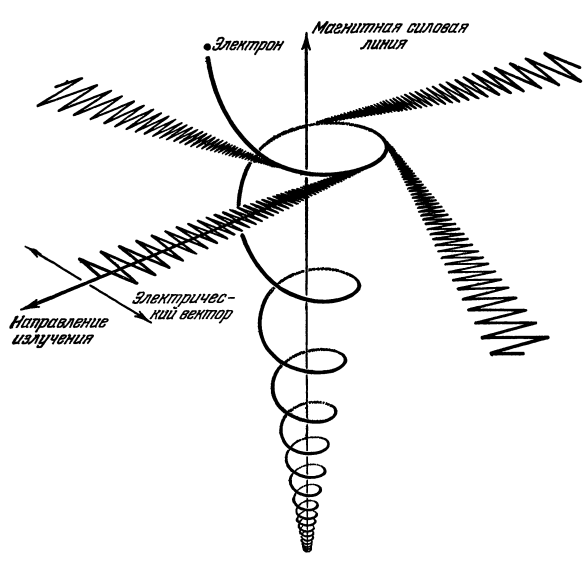
\includegraphics[width=0.3\textwidth]{synchrotron_radiation.png}
	\caption{
		К объяснению синхротронного механизма радиоизлучения.
	}
	\label{fig:synchrotron_radiation}
\end{figure}
\newpage
\subsection{Реликтовое излучение}
Реликтовое микроволновое излучение, пронизывающее весь Космос и несущее информацию о Большом взрыве. В нашу эпоху его спектр соответствует излучению абсолютно черного тела с температурой 2,725 K, так что (в соответствии с формулой Планка) максимум спектральной интенсивности приходится на длину волны 1,9 мм.

\subsection{Излучение плазмы}
Излучение плазменных волн, рожденных в атмосферах звезд и планет (обычно при участии магнитных полей). К примеру, Юпитер помимо теплового радиоизлучения выдает всплески поляризованных радиоволн, генерируемых движением заряженных частиц в верхних слоях атмосферы. Их источником служит и солнечная плазма.


\section{Синхротронное излучение (из "Essential Radio Astronomy")}
    (Формулы в системе СГС)

    На заряженную частицу (движущейся со скоростью: $ v \ll c$)
    в магнитном поле действует сила Лоренца:
    \[ 
        \vecx{F} = \frac{q [\vecx{v} \times \vecx{B}]}{c}
    \]
    
    В этом случае частица начинает двигаться по спирали вокруг магнитных линий, сила Лоренца действует перпендикулярно скорости, поэтому значение компонента скорости $v_\parallel$ параллельного линии магнитного поля остается постоянным, при этом модуль всей скорости $|\vecx{v}|$ также остается постоянной. Следовательно, значение скорости $v_\perp$, перпендикулярной магнитным линия, также остаётся постоянной. 

    Условие баланса центростремительной и магнитной сил: 
    \[ 
        m|\dot{\vecx{v}}| = m\omega^2 r = \frac{q}{c} |\vecx{v} \times \vecx{B}| = \frac{q}{c} \omega r B 
    \]
    Из него получается значение угловой частоты, с которой частица вращается вокруг линий магнитного поля в инерциальной системе отсчета движущейся со скоростью $v_\parallel$: 
    \[ 
        \omega = \frac{qB}{mc} 
    \]

    Численно, для случая электрона ($m_e \approx 9.1\times 10^{-28} $ гр, $ |e| = 4.8\times 10^{-10} $ статкулон[statC, esu](также франклин - Fr)) эта формула даёт соотношение угловой частоты от магнитного поля (B [Gauss = $10^{-5}$ T]):
    \[
        \left(\frac{\omega}{rad/s}\right) \approx 17.6\times 10^6 \cdot \left(\frac{B}{gauss}\right)
    \]

    В терминах циклической частоты ($\nu = \omega/2\pi$):
    \[
        \left(\frac{\nu}{MHz}\right) \approx 2.8 \cdot \left(\frac{B}{gauss}\right)
    \]
 
    Типичная напряженность магнитного поля межзвездного вещества (в спиральной галактике) равна $B \approx 10 [\mu G]$ (мГаусс).
    В этом случае частота равна: $\nu \approx 28 [Hz]$. 

    Магнитное поле нейтронной звезды
    $B \approx 10^{12} [G]$, что соответствует рентгеновской частоте
%-------------------------------------------------

\section{Синхротронное радиоизлучение}

Синхротронное излучение является одним из основных механизмов радиоизлучения в астрофизических объектах, таких как остатки сверхновых, активные ядра галактик и джеты. Оно возникает, когда релятивистские электроны движутся в магнитном поле, испытывая ускорение и излучая электромагнитные волны. В данном разделе представлена теоретическая основа для расчета синхротронного излучения в предположении, что этот механизм является доминирующим.

\subsection{Основные предположения}

Для упрощения расчета делаются следующие предположения:

\begin{enumerate}
    \item Механизм излучения является исключительно синхротронным. Другие механизмы, такие как тепловое излучение, обратный комптон-эффект и т.д., не рассматриваются.
    \item Функция распределения электронов по энергиям является степенной:
    \begin{equation}
        n_e(\gamma) = K \gamma^{-p},
    \end{equation}
    где $n_e(\gamma) d\gamma$ - концентрация электронов с фактором Лоренца от $\gamma$ до $\gamma + d\gamma$, $K$ - константа, определяющая концентрацию электронов, и $p$ - спектральный индекс.
    \item Магнитное поле считается однородным в пределах рассматриваемого объема, хотя его напряженность может меняться в зависимости от координат.
\end{enumerate}

\subsection{Мощность излучения одного электрона}

Мощность, излучаемая одним электроном с фактором Лоренца $\gamma$ в магнитном поле $B$, перпендикулярном направлению его движения, на частоте $\nu$, определяется как:

\begin{equation}
    P(\nu) = \frac{\sqrt{3} q_e^3 B \sin{\alpha}}{m_e c^2} F\left(\frac{\nu}{\nu_c}\right),
\end{equation}

где:
\begin{itemize}
    \item $q_e$ - элементарный заряд,
    \item $m_e$ - масса электрона,
    \item $c$ - скорость света,
    \item $\alpha$ - угол между направлением скорости электрона и магнитным полем (угол тангажа),
    \item $F(x)$ - функция, описывающая спектральное распределение синхротронного излучения (часто используется приближение в виде интеграла Макдональда),
    \item $\nu_c$ - критическая частота:
    \begin{equation}
        \nu_c = \frac{3 \gamma^2 q_e B \sin{\alpha}}{4 \pi m_e c}.
    \end{equation}
\end{itemize}

\subsection{Коэффициент излучения}

Коэффициент излучения $j_\nu$ представляет собой мощность, излучаемую единицей объема в единицу времени в единичном телесном угле на частоте $\nu$. Он получается интегрированием мощности излучения одного электрона по функции распределения электронов:

\begin{equation}
    j_\nu = \int_{\gamma_{min}}^{\gamma_{max}} P(\nu) n_e(\gamma) d\gamma,
\end{equation}

где $\gamma_{min}$ и $\gamma_{max}$ - минимальный и максимальный фактор Лоренца электронов соответственно.

Подставляя выражение для $P(\nu)$ и $n_e(\gamma)$, получаем:

\begin{equation}
     j_\nu =  \frac{\sqrt{3} q_e^3 B \sin{\alpha} K}{m_e c^2} \int_{\gamma_{min}}^{\gamma_{max}} F\left(\frac{\nu}{\nu_c}\right) \gamma^{-p}  d\gamma
\end{equation}

Вычисление этого интеграла может быть выполнено численно или с использованием приближений для функции $F(x)$.

\subsection{Самопоглощение}
В некоторых случаях необходимо учитывать эффект самопоглощения синхротронного излучения в источнике.  Это особенно важно при низких частотах и высокой концентрации электронов.

\subsection{Применимость}

Представленный расчет радиоизлучения справедлив при сделанных предположениях.  В реальных астрофизических объектах могут быть важны другие механизмы излучения, неоднородности магнитного поля, а также эффекты распространения излучения.

%-------------------------------------------------

%-------------------------------------------------

\clearpage
\sloppy
\printbibliography
%-------------------------------------------------
\end{document}

% arara: echo "@{file}"

